\documentclass{beamer}
\usetheme{Goettingen}
\usepackage{hyperref}
\begin{document}
%\nocite{voss2007essentials}
\title{Chapter 8: Maps and related tasks}  
\author{Harm Dermois \and Joris Stork}
\title{Maps and related tasks}  
\author{Harm Dubois \and Joris Stork}
\date{\today} 

\frame{\titlepage} 
\section{Blah} 
\frame{\tableofcontents} 

\section{Introduction} 

\frame{\frametitle{Introduction}
\begin{itemize}
    \item
        Maps of an environment are usually unavailable or incomplete. Even blueprints
        are not totally reliable and don't show relevant information, such as temporary
        obstacles within a building like chairs and tables.

    \item
        Additionally, available maps made for humans represent the environment
        on some abstract level that is not suited to robot interpretation or
        does not relate to robot perception or does not include information
        about objects that is relevant to the robot.

    \item
        Building a robot friendly map is very difficult and tedious.

    \item
        These considerations indicate that the robot itself is a good candidate
        for building maps that are suitable for its own use: maps built with and
        for its own sensory system.

    \item
        Robots should be able to autonomously construct, update and validate
        maps destined for robot use.
\end{itemize}
}

\frame{\frametitle{Blah}
}

\frame{\frametitle{Blah}
\begin{columns}[c]
\column{5cm}
\column{5cm}
% 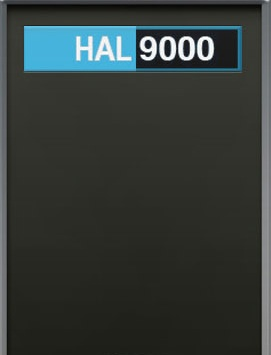
\includegraphics[width=5cm]{halsub1}
\end{columns}
}
\bibliographystyle{plain}
\bibliography{cited}
\end{document}
